%! TEX root = icml_drau.tex
\section{Experiments}
\label{sec:exp}
%! TEX root = icml_drau.tex
\begin{figure*}[ht]
	\centering
	\includegraphics[width=\textwidth]{figs_data/full_results.pdf}
	\label{fig:full_results}
	\caption{Results on a variety of environments}
\end{figure*}

The experiment set that we provide here is specifically aimed at showing that
the proposed method can operate efficiently on a wide range of time
discretization, without specific tuning, while standard deep Q-learning
approaches can't.  Our method, which is referred to as \emph{Deep Advantage
Updating}, is compared to DDPG in continuous action settings and to DQN in
discrete action settings.

In all experimental settings, we use the learning algorithm described in
alg.~\cite{alg:dau} and \TODO{supplementary, algo 1}. The variant of DDPG and DQN
used are described in the supplementary material, as well as all the hyperparameters
used.

Let us stress that quantities used are rescaled to make comparison possible. For example,
return results are given in term of macroscopic reward\footnote{This mostly amounts to scaling rewards
by a factor $\deltat$ when this scaling is not naturally done in the environment. Environment specific
details are given in the supplementary material.}, and, most notably, time elapsed is always given in
normalized epochs, i.e. the true number of epochs multiplied by the discretization timestep.

To provide qualitative results, and check that robustness to time
discretization is provided both in term of raw return results, but also in term
of convergence of approximate value function and policies to the optimal
value function and policy, we first provide results on the simple pendulum environment
provided in the openai gym classic control suite. Qualitative results are presented in
fig.~\ref{fig:full_results}.
% \begin{figure}[h]
%   \centering
%   \includegraphics[width=\columnwidth]{figs_data/cartpole_lc.png}
%   \caption{Cartpole}
%   \label{fig:cartpole-lc}
% \end{figure}

% \begin{figure}[h]
%   \centering
%   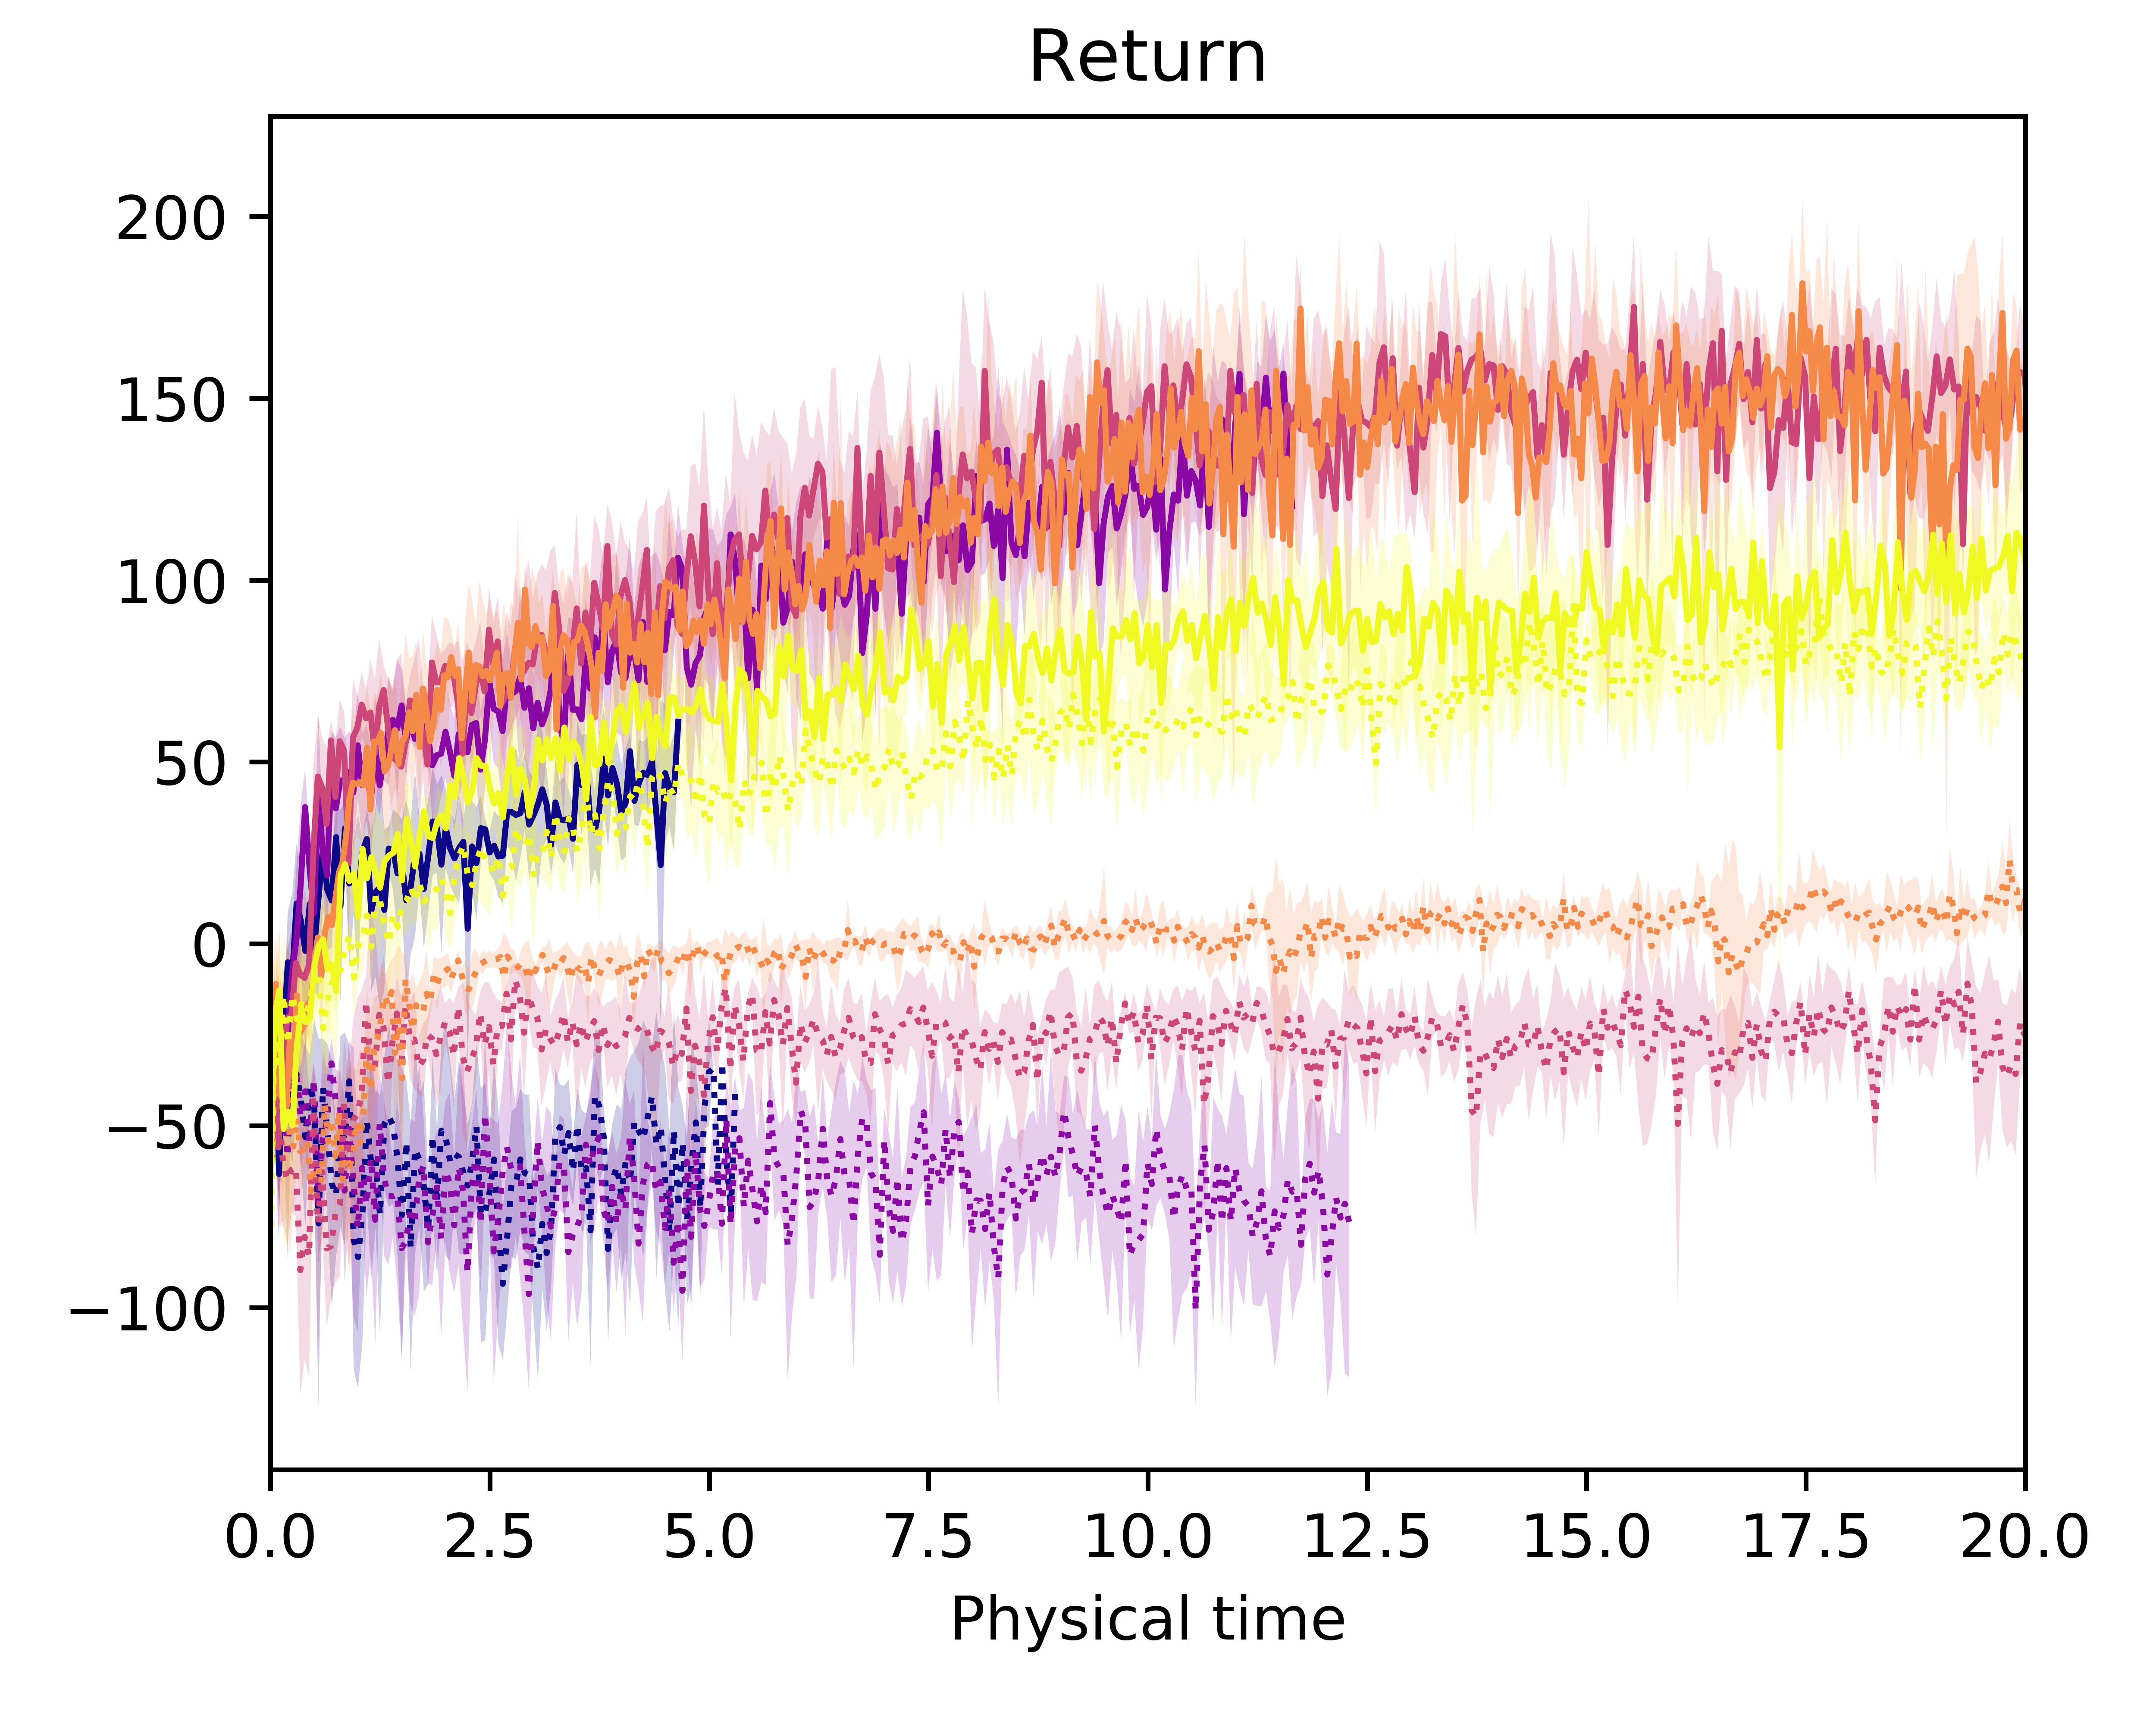
\includegraphics[width=\columnwidth]{figs_data/ant_lc.png}
%   \caption{Ant}
%   \label{fig:ant-lc}
% \end{figure}
% 
% \begin{figure}[h]
%   \centering
%   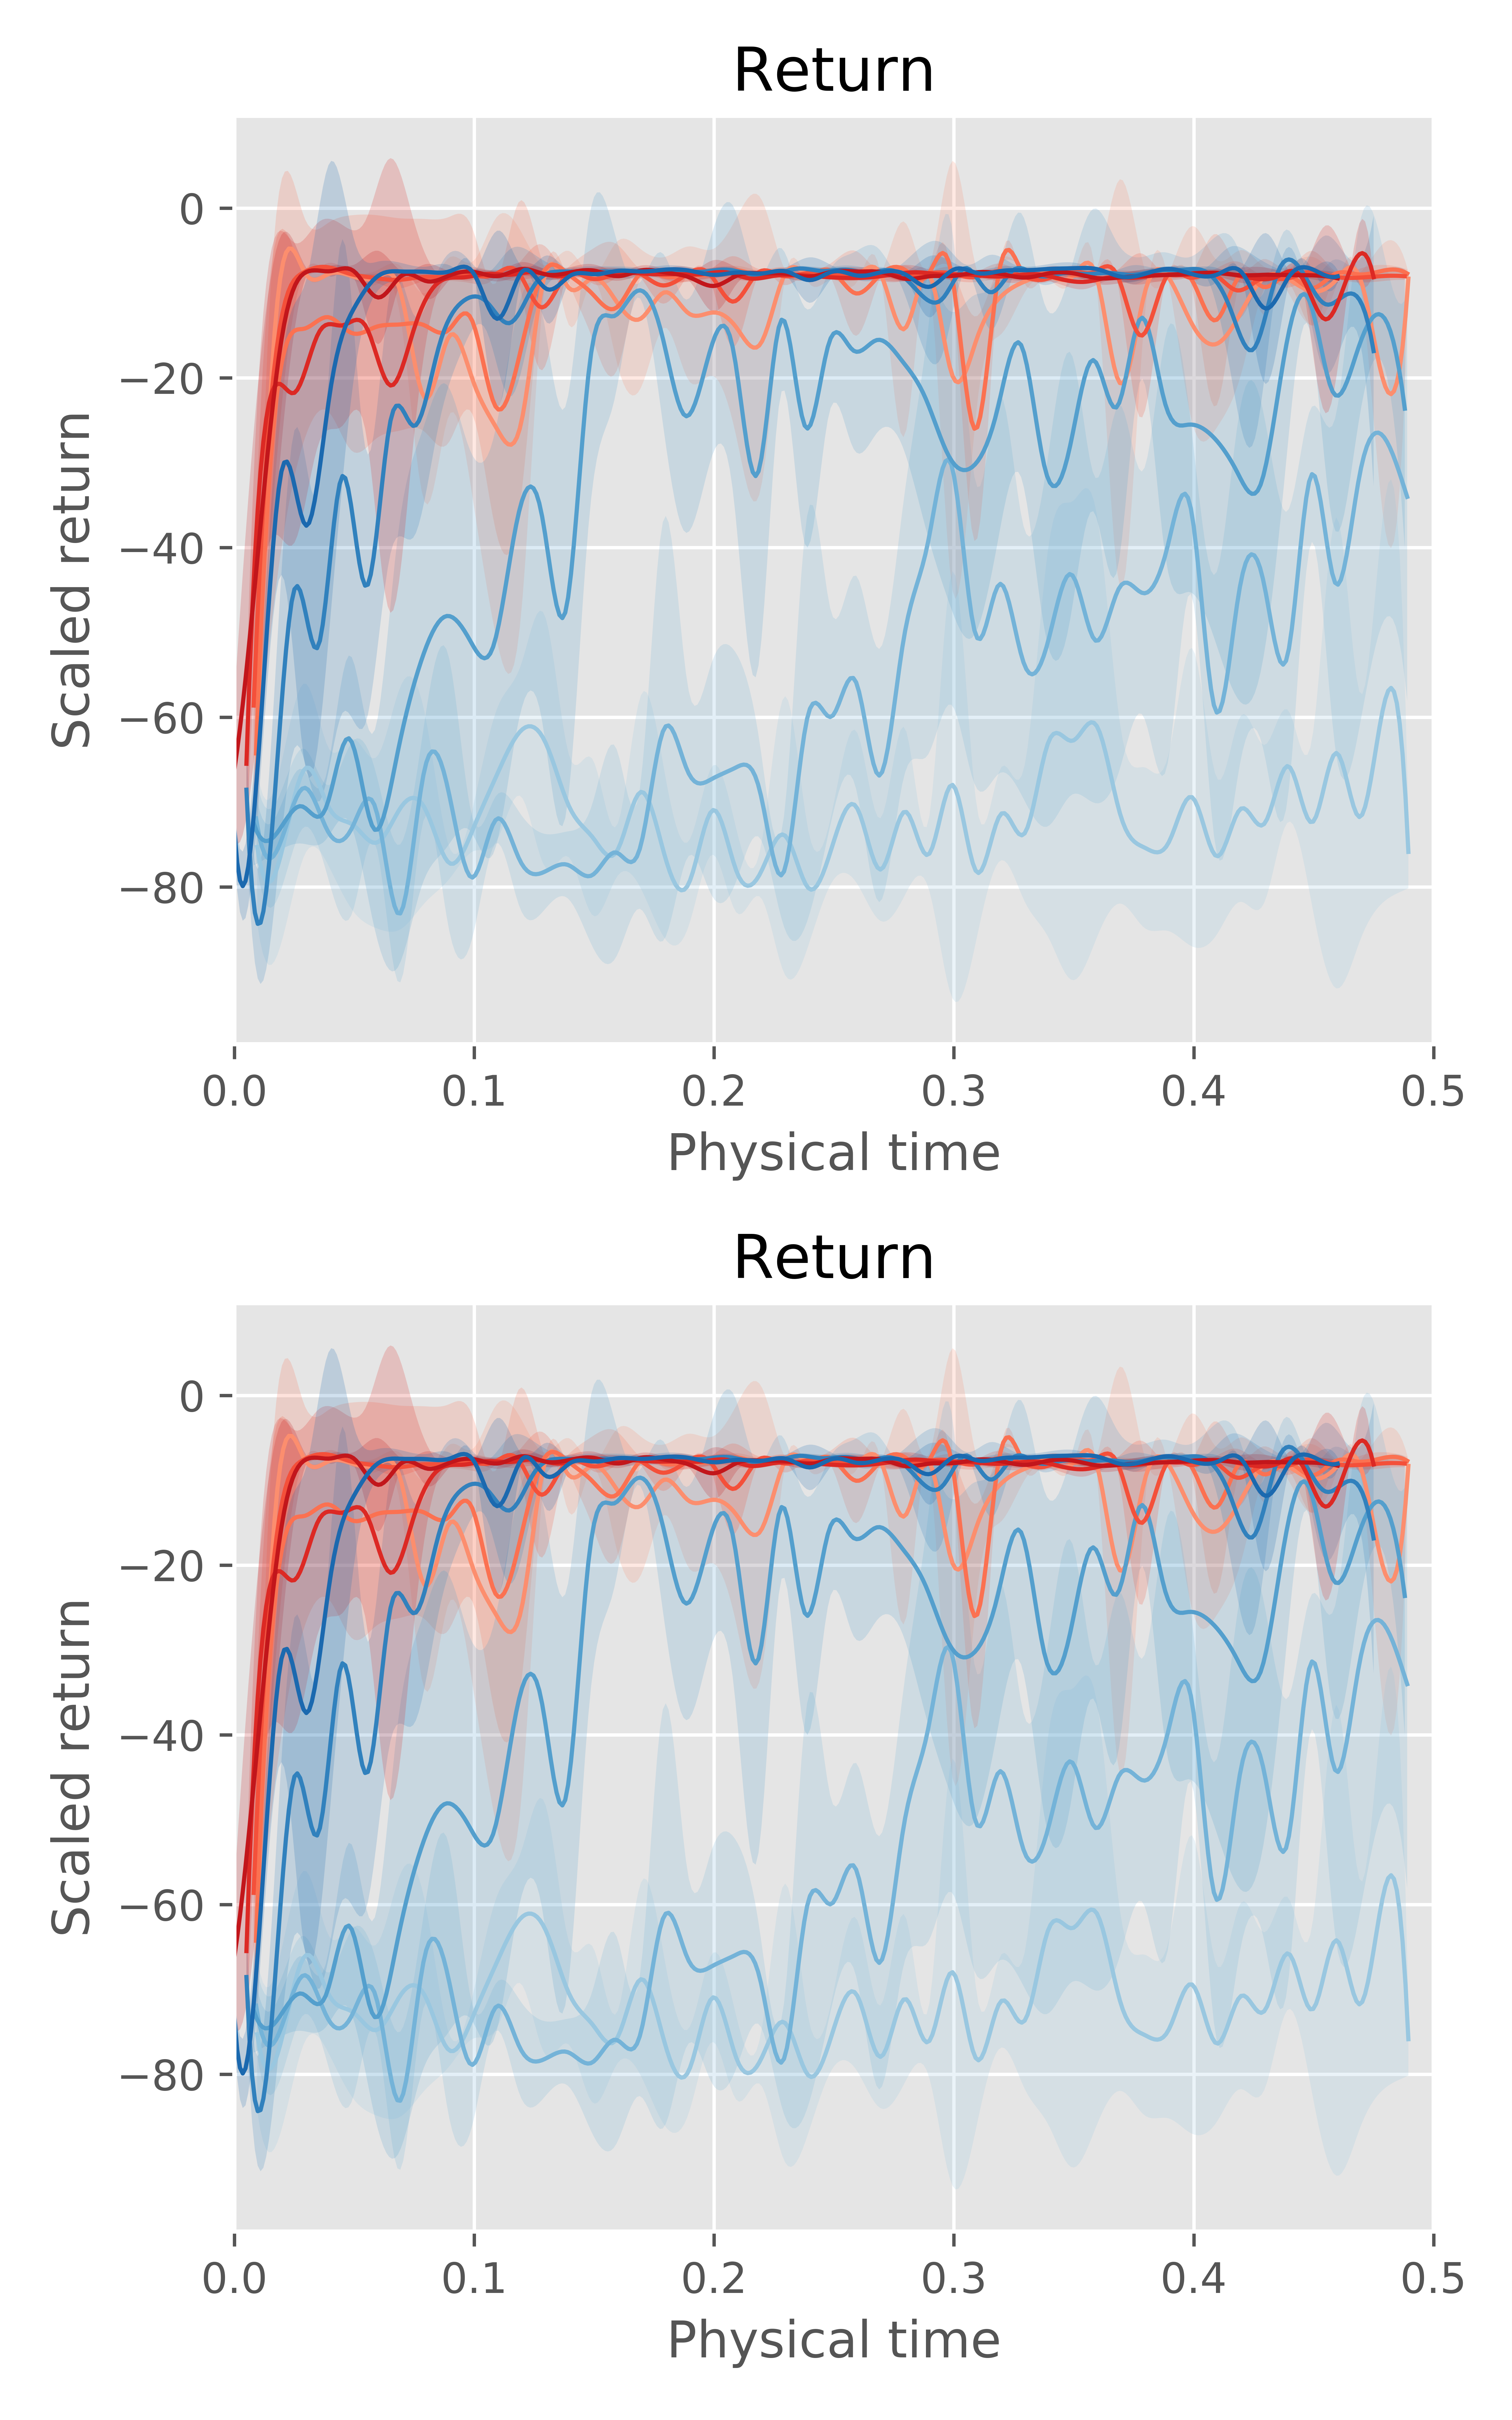
\includegraphics[width=\columnwidth]{figs_data/pendulum_lc.png}
%   \caption{Pendulum}
%   \label{fig:pendulum-lc}
% \end{figure}
